\section{Komponentenschnittstellen}

%3.1 Datentypen
\subsection{\textit{Datentypen}}
Die in Abbildung \ref{KomponentenschnittstellenDiagramm} dargestellten Datentypen werden von den Schnittstellen der eingeführten Komponenten verwendet.

Die Aufgabe des Datentyps \emph{SensorData} ist es, die Koordination mit dem \emph{Server} zu unterstützen, damit dieser feststellen kann, inwieweit eine Zielposition für einen \emph{Robot} gut zu erreichen ist. 
Dazu besitzt er als Attribute die Orientierungsrichtung im Koordinatensystem, den Batteriestatus, eine Position im räumlichen Koordinatensystem und zuletzt die mit einem eigenen Datentyp versehene \texttt{destination}. 
Wird dem \emph{Robot} nun eine neue \emph{Task} zugewiesen, erhält er damit genau diesen Datentyp \emph{Destination}, der die \emph{Position} des Patienten enthält. 
Mit dem Attribut \texttt{speed} kann der \emph{Server} außerdem genau bestimmen, mit welcher Geschwindigkeit der \emph{Robot} den Patienten anlaufen soll – also die Wichtigkeit des Einsatzes bestimmen.
\vspace{1cm}

	\begin{figure}[H]
		\centering
		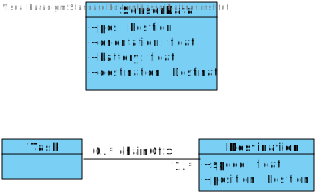
\includegraphics[width=0.42\textwidth]{img/0-Entwurf-3}
		\caption{Datentypen, die in Komponentenschnittstellen verwendet werden}
		\label{KomponentenschnittstellenDiagramm}
	\end{figure}
	\pagebreak

%3.2 Interfaces
\subsection{\textit{Interfaces}}
	%3.2.1 ISensorData
	\subsubsection{\textit{ISensorData}}
	Das Interface \textit{ISensorData} wird vom \textit{Robot} angeboten, um dem Server alle Sensordaten zu senden. 
	Der Server kann anhand dieser jederzeit feststellen, in welchem Zustand sich der \textit{Robot} befindet, um diesem dann einen \textit{Task} zuzuweisen.
	\begin{figure}[H]
	\centering
	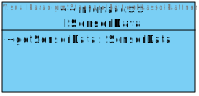
\includegraphics[width=0.4\textwidth]{img/1-Entwurf-3-1_ISensorData}
	\caption{Interface \emph{ISensorData}}
	\label{ISensorData}
	\end{figure}

	%3.2.2 ITask
	\subsubsection{\textit{ITask}}
	Das Interface \textit{ITask} wird vom \textit{Robot} angeboten, um Tasks zu erhalten. 
	Der \emph{Server} kann somit ohne Probleme dem \textit{Robot} \textit{Tasks} zuweisen. 
	Hierbei findet eine unidirektionale Kommunikation zwischen \emph{Server} und \emph{Robot} statt.
	\begin{figure}[H]
	\centering
	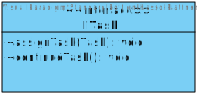
\includegraphics[width=0.4\textwidth]{img/1-Entwurf-3-1_ITask}
	\caption{Interface \emph{ITask}}
	\label{ITask}
	\end{figure}
	
	%3.2.3 IRepair
	\subsubsection{\textit{IRepair}}
	Im Falle einer Kollision, die bspw. mittels \textit{IBumperHandler} detektiert wird, benötigt die \textit{RobotUnit} manuelle Wartung, die es mittels des Interfaces \textit{IRepair} vom Server anfordern kann.
	\begin{figure}[H]
	\centering
	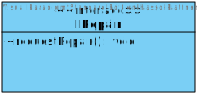
\includegraphics[width=0.4\textwidth]{img/2-Entwurf-3-IRepair}
	\caption{Interface \emph{IRepair}}
	\label{IRepair}
	\end{figure}
		
	%3.2.3 IArrivalNotification
	\subsubsection{\textit{IArrivalNotification}}
	Erreicht die \textit{RobotUnit} eine ihr eine aus dem aktuellen \textit{Task} vorgegebene \textit{Destination}, informiert sie mittels der Methode \texttt{informAboutArrival} aus dem Interface \textit{IArrivalNotification} den Server über seine Ankunft.
	\begin{figure}[H]
	\centering
	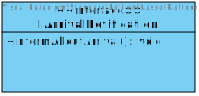
\includegraphics[width=0.4\textwidth]{img/2-Entwurf-3-IArrivalNotification}
	\caption{Interface \emph{IArrivalNotification}}
	\label{IArrivaleNotification}
	\end{figure}
